\documentclass[10pt]{beamer}

% -----------------------------------------------------------------------------
% THEME AND PACKAGES
% -----------------------------------------------------------------------------
\usetheme[progressbar=frametitle]{metropolis}
\usepackage{appendixnumberbeamer}
\usepackage{booktabs}
\usepackage{graphicx}
\usepackage{amsmath}
\usepackage{bm}
\usepackage{xcolor}
\usepackage{tikz}
\usepackage{adjustbox}
\usepackage{array}
\usetikzlibrary{arrows.meta,positioning,calc,fit,backgrounds,shapes.geometric}

\definecolor{mvblue}{HTML}{2F6BFF}
\definecolor{mvcyan}{HTML}{00A6A6}
\definecolor{mvgreen}{HTML}{2E9D57}
\definecolor{mvorange}{HTML}{D97706}
\definecolor{mvred}{HTML}{C2410C}
\definecolor{mvgray}{HTML}{F4F6F8}

\tikzset{
  flowarrow/.style={-{Latex[length=2.0mm]}, thick, draw=black!70},
  skiparrow/.style={-{Latex[length=2.0mm]}, thick, dashed, draw=black!55},
  tensor/.style={draw=black!55, rounded corners=2pt, thick, fill=mvgray,
    align=center, inner sep=3.5pt, minimum height=7mm, font=\scriptsize},
  op/.style={draw=mvblue!70!black, rounded corners=2pt, thick, fill=mvblue!8,
    align=center, inner sep=3.5pt, minimum height=8mm, font=\scriptsize},
  region/.style={draw=mvgreen!70!black, rounded corners=2pt, thick, fill=mvgreen!10,
    align=center, inner sep=3.5pt, minimum height=8mm, font=\scriptsize},
  boundary/.style={draw=mvred!75!black, rounded corners=2pt, thick, fill=mvred!9,
    align=center, inner sep=3.5pt, minimum height=8mm, font=\scriptsize},
  fpn/.style={draw=mvorange!80!black, rounded corners=2pt, thick, fill=mvorange!10,
    align=center, inner sep=3.5pt, minimum height=8mm, font=\scriptsize},
  stagebox/.style={draw=black!60, rounded corners=3pt, thick, fill=white,
    align=center, inner sep=5pt, minimum height=16mm, font=\scriptsize},
  smallnote/.style={font=\scriptsize, fill=white, inner sep=1.2pt, text=black!80}
}

% -----------------------------------------------------------------------------
% METADATA
% -----------------------------------------------------------------------------
\title{MambaRefine-CD}
\subtitle{Mamba Vision with Region-Boundary Temporal Refinement}
\author{Remote Sensing Research Group}
\institute{Multidisciplinary AI Research Center (MARC) \\ University of Peradeniya}
\date{\today}

\begin{document}

\maketitle

\begin{frame}{Table of Contents}
  \setbeamertemplate{section in toc}[sections numbered]
  \tableofcontents[hideallsubsections]
\end{frame}

% =============================================================================
\section{Introduction \& Motivation}
% =============================================================================

\begin{frame}{The Challenge of Binary Change Detection}
    Binary Change Detection (CD) in remote sensing aims to identify changed regions between bi-temporal images.
    
    \vspace{0.5em}
    \textbf{Core Challenges:}
    \begin{itemize}
        \item \textbf{Nuisance Variation:} Must be invariant to illumination shifts, seasonal changes, and shadows.
        \item \textbf{Boundary Degradation:} Errors are most visible near object boundaries, resulting in shifted, fragmented, or over-smoothed masks.
        \item \textbf{Temporal Polarity Loss:} Standard absolute differencing captures magnitude but loses direction (appearance vs. disappearance).
    \end{itemize}
\end{frame}

\begin{frame}{MambaRefine-CD: The Core Idea}
    Our architecture frames the problem as a three-question system:
    
    \vspace{0.5em}
    \begin{enumerate}
        \item \textbf{What changed?} Handled by constructing rich temporal feature differences.
        \item \textbf{Where is the changed region?} Handled by the Region Stream and an Adaptive Receptive-Field (ARF) Decoder.
        \item \textbf{Where exactly is the boundary?} Handled by the Boundary Stream and bounded residual refinement.
    \end{enumerate}
\end{frame}

% =============================================================================
\section{Architecture Overview}
% =============================================================================

\begin{frame}[plain]{MambaRefine-CD Architecture}
    \centering
    \vspace{-0.7em}
    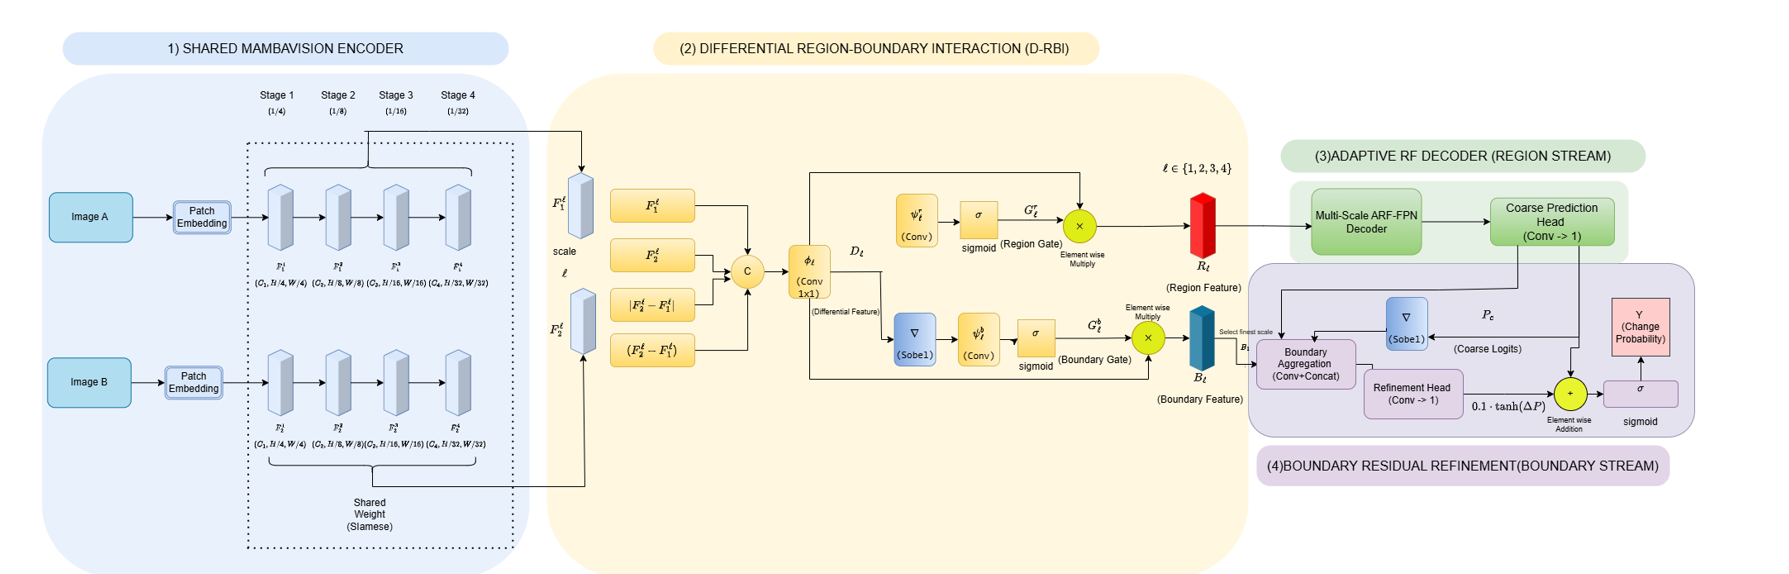
\includegraphics[width=0.99\textwidth,height=0.84\paperheight,keepaspectratio]{figures/architecture/architecture.png}
\end{frame}

\begin{frame}{High-Level Data Flow}
    \centering
    \begin{adjustbox}{max width=\textwidth,max height=0.34\textheight}
    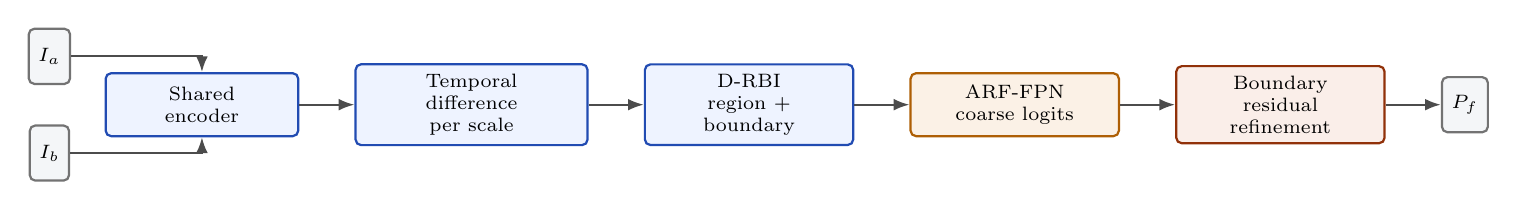
\begin{tikzpicture}[node distance=6mm and 7mm]
        \node[tensor] (ia) {\(I_a\)};
        \node[tensor, below=5mm of ia] (ib) {\(I_b\)};
        \node[op, right=of $(ia)!0.5!(ib)$, text width=22mm] (enc) {Shared\\encoder};
        \node[op, right=of enc, text width=27mm] (td) {Temporal\\difference\\per scale};
        \node[op, right=of td, text width=24mm] (drbi) {D-RBI\\region +\\boundary};
        \node[fpn, right=of drbi, text width=24mm] (arf) {ARF-FPN\\coarse logits};
        \node[boundary, right=of arf, text width=24mm] (ref) {Boundary\\residual\\refinement};
        \node[tensor, right=of ref] (pf) {\(P_f\)};

        \draw[flowarrow] (ia) -| (enc);
        \draw[flowarrow] (ib) -| (enc);
        \draw[flowarrow] (enc) -- (td);
        \draw[flowarrow] (td) -- (drbi);
        \draw[flowarrow] (drbi) -- (arf);
        \draw[flowarrow] (arf) -- (ref);
        \draw[flowarrow] (ref) -- (pf);
    \end{tikzpicture}
    \end{adjustbox}

    \vspace{0.2em}
    \scriptsize
    \begin{align*}
    \{F_a^s\}_{s=0}^{3} &= E_\theta(I_a),\qquad
    \{F_b^s\}_{s=0}^{3}=E_\theta(I_b),\\
    \Delta^s &= F_b^s-F_a^s,\qquad
    D_{\mathrm{in}}^s=[|\Delta^s|;\Delta^s]\quad \text{for \texttt{abs\_signed}},\\
    (R^s,B^s) &= \operatorname{DRBI}_s(D_{\mathrm{in}}^s),\qquad
    P_c=\operatorname{ARFFPN}(\{R^s\}_{s=0}^{3}),\\
    P_f &= P_c+0.1\tanh(\Delta P_{\mathrm{raw}}).
    \end{align*}
\end{frame}

\begin{frame}{Shared MambaVision Encoder: Four Stages}
    \centering
    \vspace{-0.2em}
    \begin{adjustbox}{max width=\textwidth,max height=0.78\textheight}
    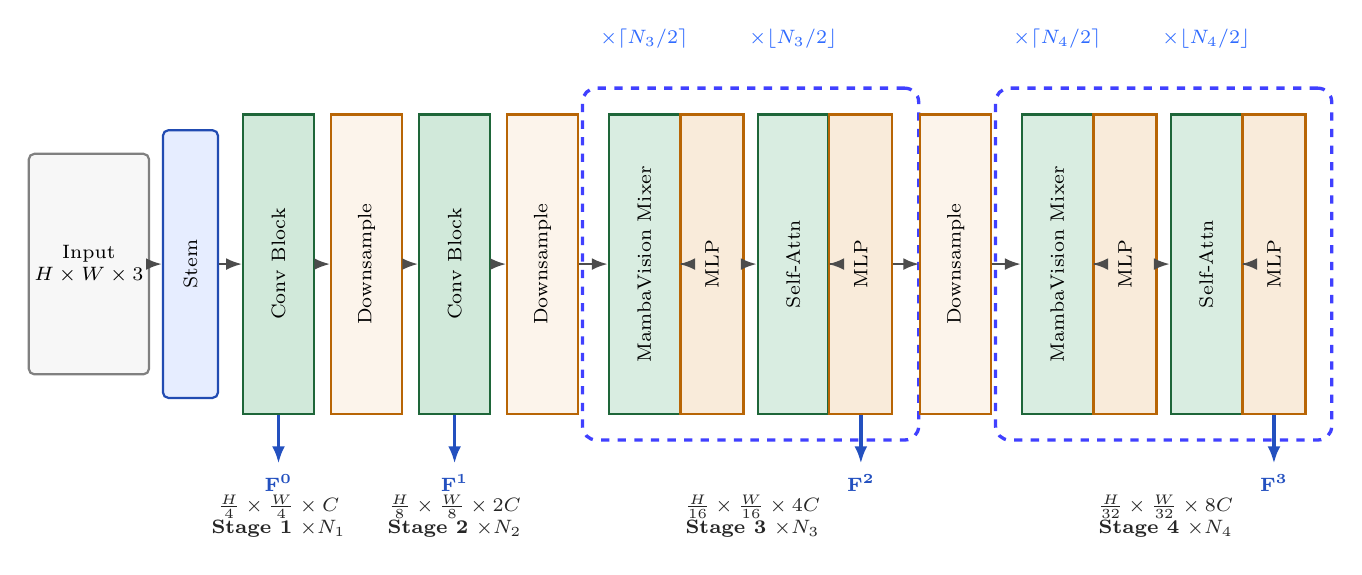
\begin{tikzpicture}[
        x=0.86mm,y=1mm,
        inputnode/.style={draw=black!50, rounded corners=2pt, thick, fill=black!3,
            minimum width=14mm, minimum height=28mm, align=center, inner sep=2pt, font=\scriptsize},
        stemblock/.style={draw=mvblue!70!black, thick, rounded corners=2pt,
            fill=mvblue!12, minimum width=7mm, minimum height=34mm,
            align=center, inner sep=1pt, font=\scriptsize},
        convblock/.style={draw=mvgreen!65!black, thick,
            fill=mvgreen!22, minimum width=9mm, minimum height=38mm,
            align=center, inner sep=1pt, font=\scriptsize},
        mixblock/.style={draw=mvgreen!65!black, thick,
            fill=mvgreen!18, minimum width=9mm, minimum height=38mm,
            align=center, inner sep=1pt, font=\scriptsize},
        mlpblock/.style={draw=mvorange!85!black, thick,
            fill=mvorange!15, minimum width=8mm, minimum height=38mm,
            align=center, inner sep=1pt, font=\scriptsize},
        downblock/.style={draw=mvorange!85!black, thick,
            fill=mvorange!8, minimum width=9mm, minimum height=38mm,
            align=center, inner sep=1pt, font=\scriptsize},
        featuretap/.style={-{Latex[length=2.2mm]}, very thick, draw=mvblue!75!black},
        stagefit/.style={draw=blue!75, very thick, dashed, rounded corners=5pt, inner sep=3.2mm},
        dimlabel/.style={font=\scriptsize, align=center, text=black!85},
        repeatlabel/.style={font=\scriptsize, text=mvblue, fill=white, inner sep=0.5pt}
    ]
        \node[inputnode] (img) at (0,0)
            {Input\\\(H\times W\times3\)};
        \node[stemblock] (stem) at (15,0) {\rotatebox{90}{Stem}};
        \node[convblock] (s1) at (28,0) {\rotatebox{90}{Conv Block}};
        \node[downblock] (d1) at (41,0) {\rotatebox{90}{Downsample}};
        \node[convblock] (s2) at (54,0) {\rotatebox{90}{Conv Block}};
        \node[downblock] (d2) at (67,0) {\rotatebox{90}{Downsample}};

        \node[mixblock] (mv3) at (82,0) {\rotatebox{90}{MambaVision Mixer}};
        \node[mlpblock] (mlp3a) at (92,0) {\rotatebox{90}{MLP}};
        \node[mixblock] (att3) at (104,0) {\rotatebox{90}{Self-Attn}};
        \node[mlpblock] (mlp3b) at (114,0) {\rotatebox{90}{MLP}};
        \node[downblock] (d3) at (128,0) {\rotatebox{90}{Downsample}};

        \node[mixblock] (mv4) at (143,0) {\rotatebox{90}{MambaVision Mixer}};
        \node[mlpblock] (mlp4a) at (153,0) {\rotatebox{90}{MLP}};
        \node[mixblock] (att4) at (165,0) {\rotatebox{90}{Self-Attn}};
        \node[mlpblock] (mlp4b) at (175,0) {\rotatebox{90}{MLP}};

        \begin{scope}[on background layer]
            \node[stagefit, fit=(mv3)(mlp3a)(att3)(mlp3b)] (g3) {};
            \node[stagefit, fit=(mv4)(mlp4a)(att4)(mlp4b)] (g4) {};
        \end{scope}

        \foreach \a/\b in {img/stem,stem/s1,s1/d1,d1/s2,s2/d2,d2/mv3,mv3/mlp3a,mlp3a/att3,att3/mlp3b,mlp3b/d3,d3/mv4,mv4/mlp4a,mlp4a/att4,att4/mlp4b}
            \draw[flowarrow] (\a) -- (\b);

        \node[repeatlabel, above=8mm of mv3] {\(\times\lceil N_3/2\rceil\)};
        \node[repeatlabel, above=8mm of att3] {\(\times\lfloor N_3/2\rfloor\)};
        \node[repeatlabel, above=8mm of mv4] {\(\times\lceil N_4/2\rceil\)};
        \node[repeatlabel, above=8mm of att4] {\(\times\lfloor N_4/2\rfloor\)};

        \draw[featuretap] (s1.south) -- ++(0,-6.2)
            node[below, font=\scriptsize, text=mvblue!75!black] {\(\mathbf{F^0}\)};
        \draw[featuretap] (s2.south) -- ++(0,-6.2)
            node[below, font=\scriptsize, text=mvblue!75!black] {\(\mathbf{F^1}\)};
        \draw[featuretap] (mlp3b.south) -- ++(0,-6.2)
            node[below, font=\scriptsize, text=mvblue!75!black] {\(\mathbf{F^2}\)};
        \draw[featuretap] (mlp4b.south) -- ++(0,-6.2)
            node[below, font=\scriptsize, text=mvblue!75!black] {\(\mathbf{F^3}\)};

        \node[dimlabel] at (28,-32)
            {\(\frac{H}{4}\times\frac{W}{4}\times C\)\\\textbf{Stage 1} \(\times N_1\)};
        \node[dimlabel] at (54,-32)
            {\(\frac{H}{8}\times\frac{W}{8}\times2C\)\\\textbf{Stage 2} \(\times N_2\)};
        \node[dimlabel] at (98,-32)
            {\(\frac{H}{16}\times\frac{W}{16}\times4C\)\\\textbf{Stage 3} \(\times N_3\)};
        \node[dimlabel] at (159,-32)
            {\(\frac{H}{32}\times\frac{W}{32}\times8C\)\\\textbf{Stage 4} \(\times N_4\)};
    \end{tikzpicture}
    \end{adjustbox}

    \vspace{0.2em}
    \scriptsize
    Encoder outputs are tapped after each stage:
    \(F^s\in\mathbb{R}^{B\times C2^s\times H/2^{s+2}\times W/2^{s+2}}\).
    For MambaVision-S: \(C=96\), \(N=(3,3,7,5)\).
\end{frame}

\begin{frame}{Encoder Block Equations}
    \small
    \begin{columns}[T,onlytextwidth]
        \begin{column}{0.43\textwidth}
            \centering
            \begin{adjustbox}{max width=\textwidth,max height=0.66\textheight}
            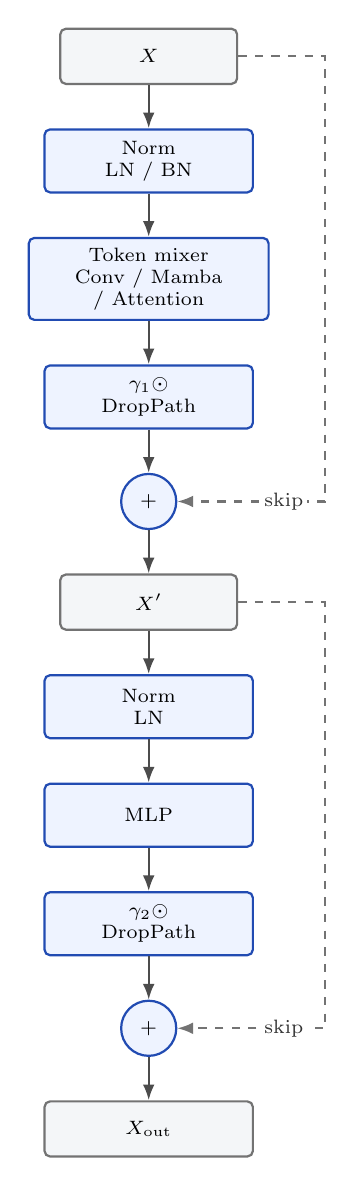
\begin{tikzpicture}[node distance=5.5mm]
                \node[tensor, text width=20mm] (x) {\(X\)};
                \node[op, below=of x, text width=24mm] (norm1) {Norm\\LN / BN};
                \node[op, below=of norm1, text width=28mm] (mix) {Token mixer\\Conv / Mamba\\/ Attention};
                \node[op, below=of mix, text width=24mm] (scale1) {\(\gamma_1\odot\)\\DropPath};
                \node[op, below=of scale1, circle, minimum size=7mm, inner sep=0pt] (add1) {\(+\)};
                \node[tensor, below=of add1, text width=20mm] (xp) {\(X'\)};
                \node[op, below=of xp, text width=24mm] (norm2) {Norm\\LN};
                \node[op, below=of norm2, text width=24mm] (mlp) {MLP};
                \node[op, below=of mlp, text width=24mm] (scale2) {\(\gamma_2\odot\)\\DropPath};
                \node[op, below=of scale2, circle, minimum size=7mm, inner sep=0pt] (add2) {\(+\)};
                \node[tensor, below=of add2, text width=24mm] (out) {\(X_{\mathrm{out}}\)};

                \draw[flowarrow] (x) -- (norm1);
                \draw[flowarrow] (norm1) -- (mix);
                \draw[flowarrow] (mix) -- (scale1);
                \draw[flowarrow] (scale1) -- (add1);
                \draw[flowarrow] (add1) -- (xp);
                \draw[flowarrow] (xp) -- (norm2);
                \draw[flowarrow] (norm2) -- (mlp);
                \draw[flowarrow] (mlp) -- (scale2);
                \draw[flowarrow] (scale2) -- (add2);
                \draw[flowarrow] (add2) -- (out);

                \draw[skiparrow] (x.east) -- ++(11mm,0) |- node[smallnote, pos=0.72, right] {skip} (add1.east);
                \draw[skiparrow] (xp.east) -- ++(11mm,0) |- node[smallnote, pos=0.72, right] {skip} (add2.east);
            \end{tikzpicture}
            \end{adjustbox}
        \end{column}
        \begin{column}{0.54\textwidth}
            \begin{align*}
            U &= \mathcal{M}(\operatorname{Norm}_1(X)),\\
            X' &= X+\operatorname{DropPath}(\gamma_1\odot U),\\
            V &= \operatorname{MLP}(\operatorname{Norm}_2(X')),\\
            X_{\mathrm{out}} &= X'+\operatorname{DropPath}(\gamma_2\odot V).
            \end{align*}
            \vspace{-0.2em}
            \scriptsize
            \[
            \mathcal{M}=
            \begin{cases}
            \text{convolutional residual stack}, & \text{stages 1--2},\\
            \text{MambaVision mixer or self-attention}, & \text{stages 3--4}.
            \end{cases}
            \]
            The block is pre-normalized and residual at both the token-mixing and MLP sublayers.
        \end{column}
    \end{columns}
\end{frame}

\begin{frame}{MambaVision Mixer Inside Stages 2--3}
    \centering
    \begin{adjustbox}{max width=\textwidth,max height=0.58\textheight}
    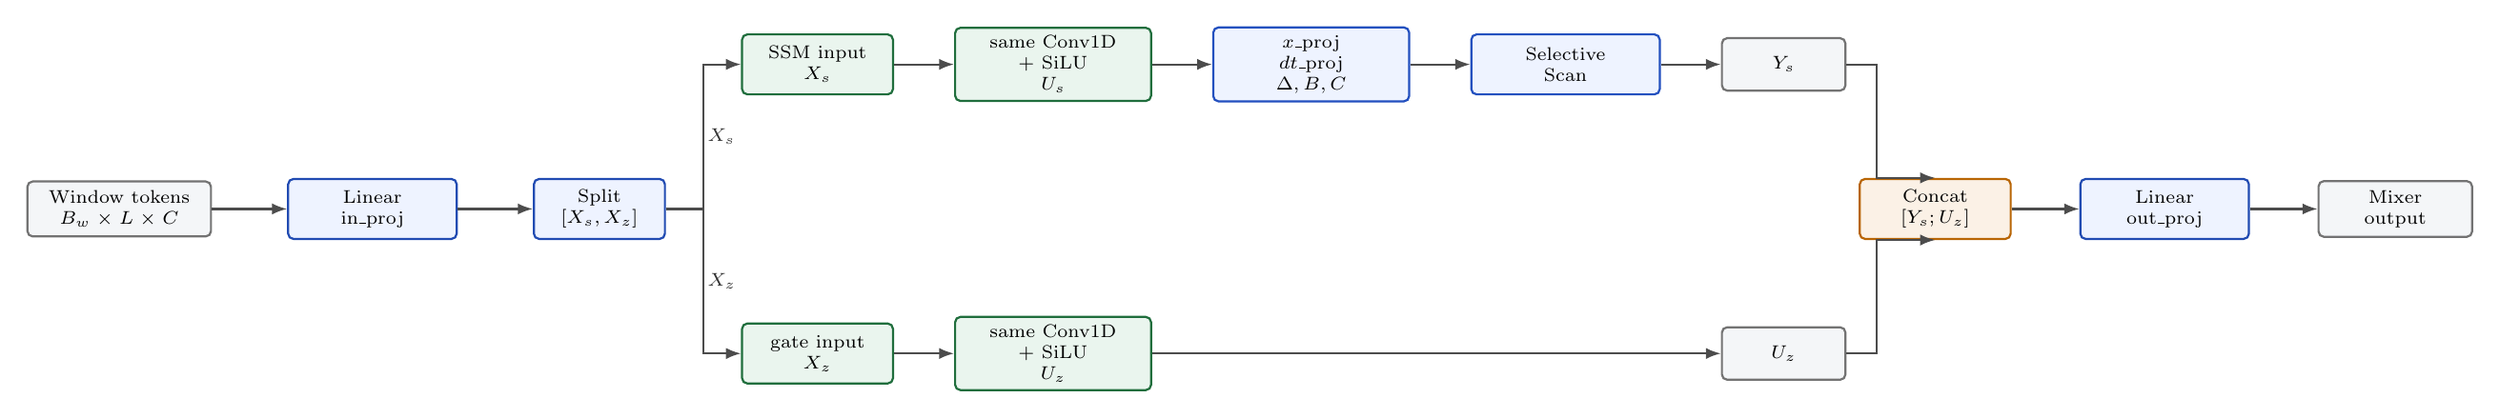
\begin{tikzpicture}[
        node distance=6mm and 8mm,
        branch/.style={draw=mvgreen!70!black, rounded corners=2pt, thick,
            fill=mvgreen!10, align=center, inner sep=3pt, minimum height=8mm,
            font=\scriptsize},
        scanop/.style={draw=mvblue!75!black, rounded corners=2pt, thick,
            fill=mvblue!8, align=center, inner sep=3pt, minimum height=8mm,
            font=\scriptsize},
        merge/.style={draw=mvorange!85!black, rounded corners=2pt, thick,
            fill=mvorange!10, align=center, inner sep=3pt, minimum height=8mm,
            font=\scriptsize}
    ]
        \node[tensor, text width=22mm] (x) at (0,0) {Window tokens\\\(B_w\times L\times C\)};
        \node[op, right=10mm of x, text width=20mm] (proj) {Linear\\in\_proj};
        \node[op, right=10mm of proj, text width=15mm] (split) {Split\\\([X_s,X_z]\)};

        \node[branch, above right=11mm and 10mm of split, text width=18mm] (xs) {SSM input\\\(X_s\)};
        \node[branch, right=8mm of xs, text width=24mm] (ssmconv) {same Conv1D\\+ SiLU\\\(U_s\)};
        \node[scanop, right=8mm of ssmconv, text width=24mm] (params) {\(x\_\)proj\\\(dt\_\)proj\\\(\Delta,B,C\)};
        \node[scanop, right=8mm of params, text width=23mm] (scan) {Selective\\Scan};
        \node[tensor, right=8mm of scan, text width=14mm] (ys) {\(Y_s\)};

        \node[branch, below right=11mm and 10mm of split, text width=18mm] (xz) {gate input\\\(X_z\)};
        \node[branch, right=8mm of xz, text width=24mm] (sym) {same Conv1D\\+ SiLU\\\(U_z\)};
        \node[tensor, text width=14mm] (uz) at (ys |- sym) {\(U_z\)};

        \node[merge, right=10mm of $(ys)!0.5!(uz)$, text width=18mm] (cat) {Concat\\\([Y_s;U_z]\)};
        \node[op, right=9mm of cat, text width=20mm] (outproj) {Linear\\out\_proj};
        \node[tensor, right=9mm of outproj, text width=18mm] (y) {Mixer\\output};

        \draw[flowarrow] (x) -- (proj);
        \draw[flowarrow] (proj) -- (split);
        \draw[flowarrow] (split.east) -- ++(5mm,0) |- node[smallnote, pos=0.25, right] {\(X_s\)} (xs.west);
        \draw[flowarrow] (split.east) -- ++(5mm,0) |- node[smallnote, pos=0.25, right] {\(X_z\)} (xz.west);
        \draw[flowarrow] (xs) -- (ssmconv);
        \draw[flowarrow] (ssmconv) -- (params);
        \draw[flowarrow] (params) -- (scan);
        \draw[flowarrow] (scan) -- (ys);
        \draw[flowarrow] (xz) -- (sym);
        \draw[flowarrow] (sym) -- (uz);
        \draw[flowarrow] (ys.east) -- ++(4mm,0) |- (cat.north);
        \draw[flowarrow] (uz.east) -- ++(4mm,0) |- (cat.south);
        \draw[flowarrow] (cat) -- (outproj);
        \draw[flowarrow] (outproj) -- (y);
    \end{tikzpicture}
    \end{adjustbox}

    \vspace{0.2em}
    \scriptsize
    \begin{align*}
    [X_s,X_z] &= \operatorname{split}(W_{\mathrm{in}}X),&
    U_s &= \operatorname{SiLU}(\operatorname{Conv1D}_{\mathrm{same}}(X_s)),\\
    U_z &= \operatorname{SiLU}(\operatorname{Conv1D}_{\mathrm{same}}(X_z)),&
    [\Delta_k,B_k,C_k] &= W_x U_{s,k},\\
    h_k &= \bar{A}_k h_{k-1}+\bar{B}_k U_{s,k},&
    Y &= W_{\mathrm{out}}[Y_s;U_z].
    \end{align*}
\end{frame}

% =============================================================================
\section{Differential Region-Boundary Interaction (D-RBI)}
% =============================================================================

\begin{frame}{D-RBI 2.1: Difference Input and 1x1 Projection}
    \centering
    \begin{adjustbox}{max width=\textwidth,max height=0.56\textheight}
    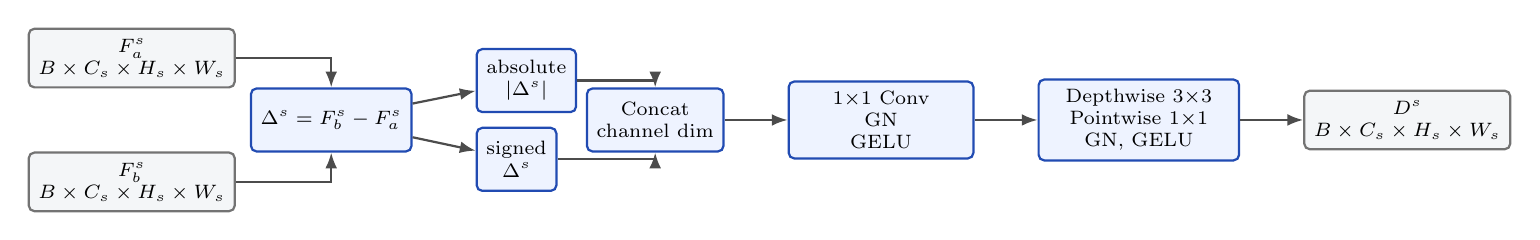
\begin{tikzpicture}[node distance=7mm and 8mm]
        \node[tensor] (fa) {\(F_a^s\)\\\(B\times C_s\times H_s\times W_s\)};
        \node[tensor, below=8mm of fa] (fb) {\(F_b^s\)\\\(B\times C_s\times H_s\times W_s\)};
        \node[op, right=15mm of $(fa)!0.5!(fb)$] (diff) {\(\Delta^s=F_b^s-F_a^s\)};
        \node[op, right=of diff, yshift=5mm] (abs) {absolute\\\(|\Delta^s|\)};
        \node[op, right=of diff, yshift=-5mm] (signed) {signed\\\(\Delta^s\)};
        \node[op, right=22mm of diff] (concat) {Concat\\channel dim};
        \node[op, right=of concat, text width=21mm] (proj) {\(1{\times}1\) Conv\\GN\\GELU};
        \node[op, right=of proj, text width=23mm] (spatial) {Depthwise \(3{\times}3\)\\Pointwise \(1{\times}1\)\\GN, GELU};
        \node[tensor, right=of spatial] (d) {\(D^s\)\\\(B\times C_s\times H_s\times W_s\)};

        \draw[flowarrow] (fa) -| (diff);
        \draw[flowarrow] (fb) -| (diff);
        \draw[flowarrow] (diff) -- (abs);
        \draw[flowarrow] (diff) -- (signed);
        \draw[flowarrow] (abs) -| (concat);
        \draw[flowarrow] (signed) -| (concat);
        \draw[flowarrow] (concat) -- (proj);
        \draw[flowarrow] (proj) -- (spatial);
        \draw[flowarrow] (spatial) -- (d);
    \end{tikzpicture}
    \end{adjustbox}

    \vspace{0.2em}
    \scriptsize
    \begin{align*}
    \Delta^s &= F_b^s-F_a^s,\qquad
    D_{\mathrm{in}}^s=[|\Delta^s|;\Delta^s]\quad \text{for default \texttt{abs\_signed}},\\
    \hat{D}^s &= \operatorname{GELU}(\operatorname{GN}(W_p^{1\times1}*D_{\mathrm{in}}^s)),\\
    D^s &= \operatorname{GELU}(\operatorname{GN}(W_{\mathrm{pw}}^{1\times1}*(W_{\mathrm{dw}}^{3\times3}*\hat{D}^s))).
    \end{align*}
\end{frame}

\begin{frame}{D-RBI 2.2: Regional Feature Path}
    \centering
    \begin{adjustbox}{max width=\textwidth,max height=0.40\textheight}
    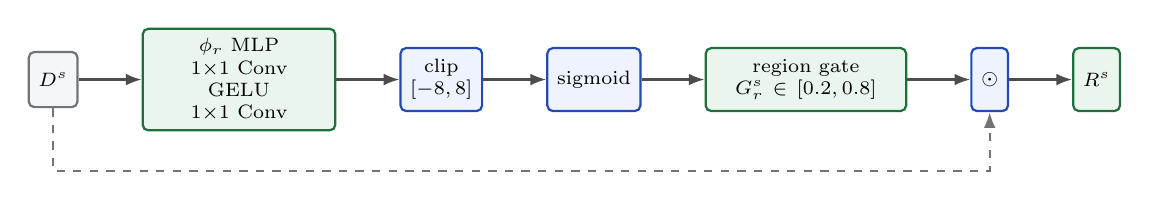
\begin{tikzpicture}[node distance=7mm and 8mm]
        \node[tensor] (d) {\(D^s\)};
        \node[region, right=of d, text width=22mm] (phi) {\(\phi_r\) MLP\\\(1{\times}1\) Conv\\GELU\\\(1{\times}1\) Conv};
        \node[op, right=of phi] (clip) {clip\\\([-8,8]\)};
        \node[op, right=of clip] (sig) {sigmoid};
        \node[region, right=of sig, text width=23mm] (gate) {region gate\\\(G_r^s\in[0.2,0.8]\)};
        \node[op, right=of gate] (mul) {\(\odot\)};
        \node[region, right=of mul] (r) {\(R^s\)};

        \draw[flowarrow] (d) -- (phi);
        \draw[flowarrow] (phi) -- (clip);
        \draw[flowarrow] (clip) -- (sig);
        \draw[flowarrow] (sig) -- (gate);
        \draw[flowarrow] (gate) -- (mul);
        \draw[skiparrow] (d.south) -- ++(0,-8mm) -| (mul.south);
        \draw[flowarrow] (mul) -- (r);
    \end{tikzpicture}
    \end{adjustbox}

    \vspace{0.2em}
    \scriptsize
    \begin{align*}
    H_r^s &= \operatorname{GELU}(W_{r,1}^{1\times1}*D^s+b_{r,1}),\\
    \phi_r(D^s) &= W_{r,2}^{1\times1}*H_r^s+b_{r,2},\\
    G_r^s &= 0.2+0.6\,\sigma(\operatorname{clip}(\phi_r(D^s),-8,8)),\qquad
    R^s=D^s\odot G_r^s.
    \end{align*}
\end{frame}

\begin{frame}{D-RBI 2.3: Boundary Feature Path}
    \centering
    \begin{adjustbox}{max width=\textwidth,max height=0.42\textheight}
    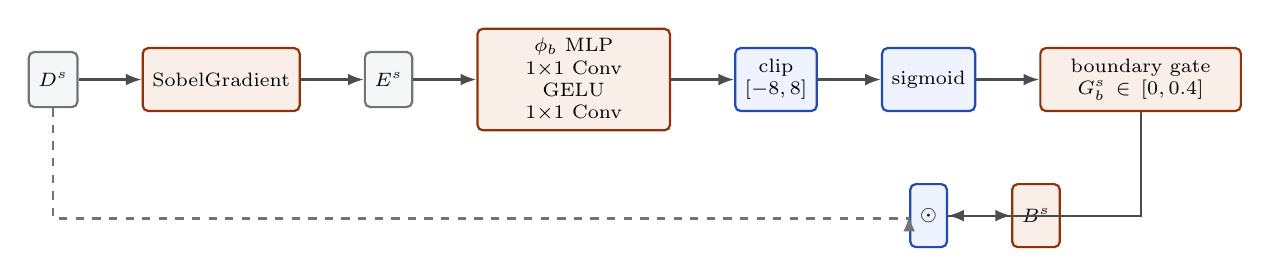
\begin{tikzpicture}[node distance=7mm and 8mm]
        \node[tensor] (d) {\(D^s\)};
        \node[boundary, right=of d] (sob) {SobelGradient};
        \node[tensor, right=of sob] (edge) {\(E^s\)};
        \node[boundary, right=of edge, text width=22mm] (phi) {\(\phi_b\) MLP\\\(1{\times}1\) Conv\\GELU\\\(1{\times}1\) Conv};
        \node[op, right=of phi] (clip) {clip\\\([-8,8]\)};
        \node[op, right=of clip] (sig) {sigmoid};
        \node[boundary, right=of sig, text width=23mm] (gate) {boundary gate\\\(G_b^s\in[0,0.4]\)};
        \node[op, below=9mm of sig] (mul) {\(\odot\)};
        \node[boundary, right=of mul] (b) {\(B^s\)};

        \draw[flowarrow] (d) -- (sob);
        \draw[flowarrow] (sob) -- (edge);
        \draw[flowarrow] (edge) -- (phi);
        \draw[flowarrow] (phi) -- (clip);
        \draw[flowarrow] (clip) -- (sig);
        \draw[flowarrow] (sig) -- (gate);
        \draw[flowarrow] (gate.south) |- (mul);
        \draw[skiparrow] (d.south) -- ++(0,-14mm) -| (mul.west);
        \draw[flowarrow] (mul) -- (b);
    \end{tikzpicture}
    \end{adjustbox}

    \vspace{0.15em}
    \scriptsize
    \begin{align*}
    E^s &= \operatorname{SobelGradient}(D^s),\qquad
    H_b^s=\operatorname{GELU}(W_{b,1}^{1\times1}*E^s+b_{b,1}),\\
    \phi_b(E^s) &= W_{b,2}^{1\times1}*H_b^s+b_{b,2},\\
    G_b^s &= 0.4\,\sigma(\operatorname{clip}(\phi_b(E^s),-8,8)),\qquad
    B^s=D^s\odot G_b^s.
    \end{align*}
\end{frame}

\begin{frame}{D-RBI 2.4: Sobel Block}
    \begin{columns}[T,onlytextwidth]
        \begin{column}{0.49\textwidth}
            \centering
            \begin{adjustbox}{max width=\textwidth,max height=0.56\textheight}
            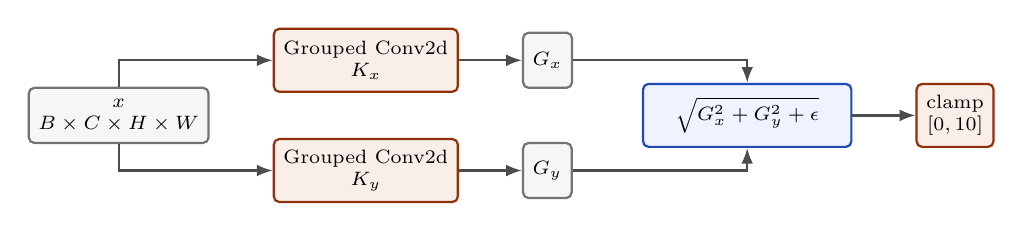
\begin{tikzpicture}[node distance=7mm and 8mm]
                \node[tensor] (x) {\(x\)\\\(B\times C\times H\times W\)};
                \node[boundary, right=of x, yshift=7mm] (kx) {Grouped Conv2d\\\(K_x\)};
                \node[boundary, right=of x, yshift=-7mm] (ky) {Grouped Conv2d\\\(K_y\)};
                \node[tensor, right=of kx] (gx) {\(G_x\)};
                \node[tensor, right=of ky] (gy) {\(G_y\)};
                \node[op, right=12mm of $(gx)!0.5!(gy)$, text width=24mm] (mag) {\(\sqrt{G_x^2+G_y^2+\epsilon}\)};
                \node[boundary, right=of mag] (out) {clamp\\\([0,10]\)};

                \draw[flowarrow] (x) |- (kx);
                \draw[flowarrow] (x) |- (ky);
                \draw[flowarrow] (kx) -- (gx);
                \draw[flowarrow] (ky) -- (gy);
                \draw[flowarrow] (gx) -| (mag);
                \draw[flowarrow] (gy) -| (mag);
                \draw[flowarrow] (mag) -- (out);
            \end{tikzpicture}
            \end{adjustbox}
        \end{column}
        \begin{column}{0.48\textwidth}
            \scriptsize
            \[
            K_x=\begin{bmatrix}-1&0&1\\-2&0&2\\-1&0&1\end{bmatrix},
            \qquad
            K_y=\begin{bmatrix}-1&-2&-1\\0&0&0\\1&2&1\end{bmatrix}
            \]
            \[
            G_x=x*K_x,\qquad G_y=x*K_y
            \]
            \[
            \operatorname{SobelGradient}(x)=
            \operatorname{clip}\left(\sqrt{G_x^2+G_y^2+10^{-6}},0,10\right).
            \]
        \end{column}
    \end{columns}
\end{frame}

\begin{frame}{D-RBI 2.5: \(\phi_r\) and \(\phi_b\) Gate Blocks}
    \centering
    \begin{adjustbox}{max width=\textwidth,max height=0.52\textheight}
    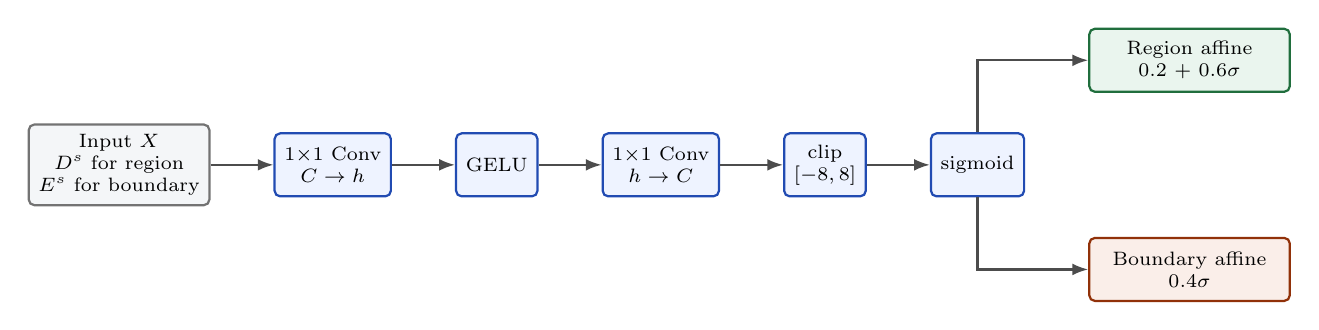
\begin{tikzpicture}[node distance=7mm and 8mm]
        \node[tensor] (x) {Input \(X\)\\\(D^s\) for region\\\(E^s\) for boundary};
        \node[op, right=of x] (c1) {\(1{\times}1\) Conv\\\(C\to h\)};
        \node[op, right=of c1] (gelu) {GELU};
        \node[op, right=of gelu] (c2) {\(1{\times}1\) Conv\\\(h\to C\)};
        \node[op, right=of c2] (clip) {clip\\\([-8,8]\)};
        \node[op, right=of clip] (sig) {sigmoid};
        \node[region, above right=5mm and 8mm of sig, text width=23mm] (rg) {Region affine\\\(0.2+0.6\sigma\)};
        \node[boundary, below right=5mm and 8mm of sig, text width=23mm] (bg) {Boundary affine\\\(0.4\sigma\)};

        \draw[flowarrow] (x) -- (c1);
        \draw[flowarrow] (c1) -- (gelu);
        \draw[flowarrow] (gelu) -- (c2);
        \draw[flowarrow] (c2) -- (clip);
        \draw[flowarrow] (clip) -- (sig);
        \draw[flowarrow] (sig) |- (rg);
        \draw[flowarrow] (sig) |- (bg);
    \end{tikzpicture}
    \end{adjustbox}

    \vspace{0.2em}
    \small
    \[
    h=\max(\lfloor 0.25C\rfloor,1),\quad
    \phi(X)=W_2^{1\times1}*\operatorname{GELU}(W_1^{1\times1}*X+b_1)+b_2.
    \]
    \[
    G_r=0.2+0.6\sigma(\operatorname{clip}(\phi_r,-8,8)),\qquad
    G_b=0.4\sigma(\operatorname{clip}(\phi_b,-8,8)).
    \]
\end{frame}

% =============================================================================
\section{Decoding \& Refinement}
% =============================================================================

\begin{frame}{Multi-Scale ARF-FPN Decoder}
    \begin{columns}[T,onlytextwidth]
        \begin{column}{0.58\textwidth}
            \centering
            \begin{adjustbox}{max width=\textwidth,max height=0.64\textheight}
            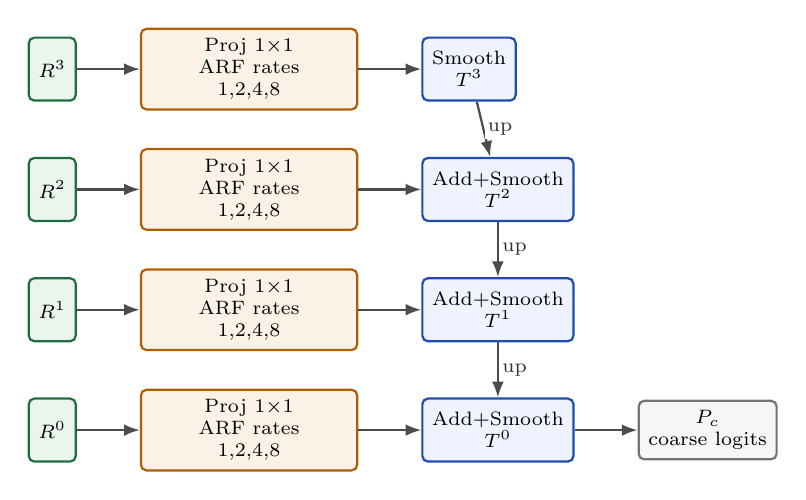
\begin{tikzpicture}[node distance=6mm and 8mm]
                \node[region] (r3) {\(R^3\)};
                \node[region, below=7mm of r3] (r2) {\(R^2\)};
                \node[region, below=7mm of r2] (r1) {\(R^1\)};
                \node[region, below=7mm of r1] (r0) {\(R^0\)};

                \node[fpn, right=of r3, text width=25mm] (p3) {Proj \(1{\times}1\)\\ARF rates\\1,2,4,8};
                \node[fpn, right=of r2, text width=25mm] (p2) {Proj \(1{\times}1\)\\ARF rates\\1,2,4,8};
                \node[fpn, right=of r1, text width=25mm] (p1) {Proj \(1{\times}1\)\\ARF rates\\1,2,4,8};
                \node[fpn, right=of r0, text width=25mm] (p0) {Proj \(1{\times}1\)\\ARF rates\\1,2,4,8};

                \node[op, right=of p3] (t3) {Smooth\\\(T^3\)};
                \node[op, right=of p2] (t2) {Add+Smooth\\\(T^2\)};
                \node[op, right=of p1] (t1) {Add+Smooth\\\(T^1\)};
                \node[op, right=of p0] (t0) {Add+Smooth\\\(T^0\)};
                \node[tensor, right=of t0] (pc) {\(P_c\)\\coarse logits};

                \foreach \a/\b in {r3/p3,r2/p2,r1/p1,r0/p0,p3/t3,p2/t2,p1/t1,p0/t0,t0/pc}
                    \draw[flowarrow] (\a) -- (\b);
                \draw[flowarrow] (t3) -- node[smallnote, right] {up} (t2);
                \draw[flowarrow] (t2) -- node[smallnote, right] {up} (t1);
                \draw[flowarrow] (t1) -- node[smallnote, right] {up} (t0);
            \end{tikzpicture}
            \end{adjustbox}
        \end{column}
        \begin{column}{0.39\textwidth}
            \scriptsize
            \begin{align*}
            \tilde{R}^s &= \operatorname{Proj}_{s}^{1\times1}(R^s),\\
            Z_{s,r} &= \operatorname{ConvNormGELU}_{3\times3,d=r}(\tilde{R}^s),\\
            \alpha_s &= \operatorname{softmax}(\operatorname{MLP}(\operatorname{GAP}(\tilde{R}^s))),\\
            P^s &= \sum_{r\in\{1,2,4,8\}}\alpha_{s,r}Z_{s,r},\\
            T^3 &= \operatorname{Smooth}_3(P^3),\\
            T^s &= \operatorname{Smooth}_s(P^s+\operatorname{Up}(T^{s+1})),\\
            P_c &= \operatorname{Up}(\operatorname{Head}(T^0)).
            \end{align*}
        \end{column}
    \end{columns}
\end{frame}

\begin{frame}{Coarse Prediction Head}
    \centering
    \begin{adjustbox}{max width=\textwidth,max height=0.42\textheight}
    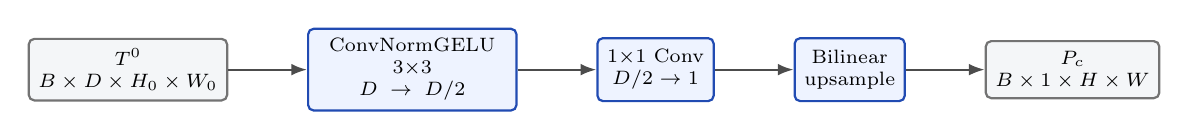
\begin{tikzpicture}[node distance=8mm and 10mm]
        \node[tensor] (t0) {\(T^0\)\\\(B\times D\times H_0\times W_0\)};
        \node[op, right=of t0, text width=24mm] (conv) {ConvNormGELU\\\(3{\times}3\)\\\(D\to D/2\)};
        \node[op, right=of conv] (c1) {\(1{\times}1\) Conv\\\(D/2\to1\)};
        \node[op, right=of c1] (up) {Bilinear\\upsample};
        \node[tensor, right=of up] (pc) {\(P_c\)\\\(B\times1\times H\times W\)};
        \draw[flowarrow] (t0) -- (conv);
        \draw[flowarrow] (conv) -- (c1);
        \draw[flowarrow] (c1) -- (up);
        \draw[flowarrow] (up) -- (pc);
    \end{tikzpicture}
    \end{adjustbox}

    \vspace{0.4em}
    \small
    \[
    H_c=\operatorname{GELU}(\operatorname{GN}(W_h^{3\times3}*T^0)),\quad
    \ell_c=W_o^{1\times1}*H_c+b_o,\quad
    P_c=\operatorname{Up}(\ell_c;H,W).
    \]
\end{frame}

\begin{frame}{Boundary Residual Refinement: Full Block}
    \centering
    \begin{adjustbox}{max width=\textwidth,max height=0.61\textheight}
    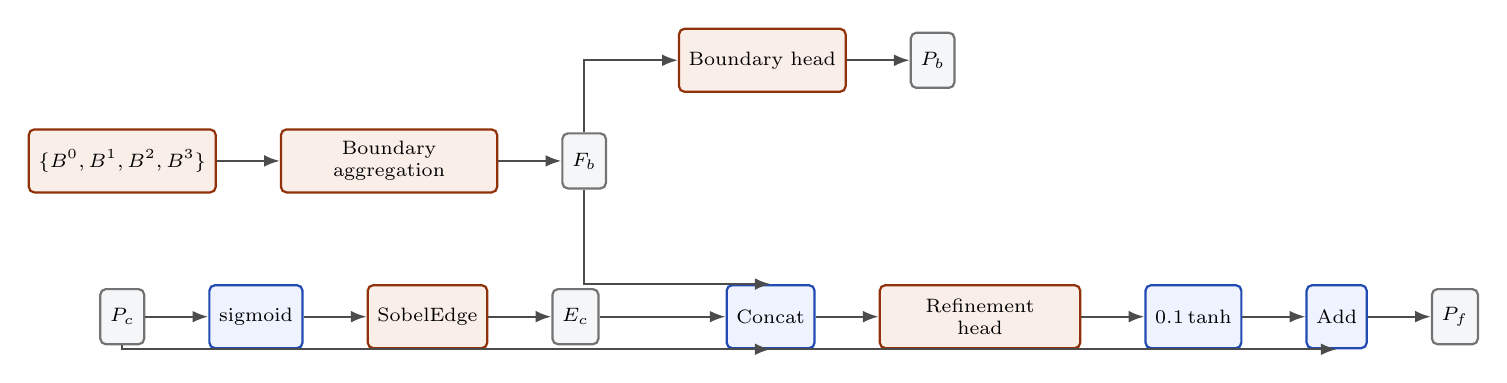
\begin{tikzpicture}[node distance=7mm and 8mm]
        \node[boundary] (bs) {\(\{B^0,B^1,B^2,B^3\}\)};
        \node[boundary, right=of bs, text width=25mm] (agg) {Boundary\\aggregation};
        \node[tensor, right=of agg] (bf) {\(F_b\)};
        \node[boundary, above right=5mm and 9mm of bf] (bh) {Boundary head};
        \node[tensor, right=of bh] (blog) {\(P_b\)};

        \node[tensor, below=12mm of bs] (pc) {\(P_c\)};
        \node[op, right=of pc] (sig) {sigmoid};
        \node[boundary, right=of sig] (sob) {SobelEdge};
        \node[tensor, right=of sob] (edge) {\(E_c\)};
        \node[op, right=16mm of edge] (cat) {Concat};
        \node[boundary, right=of cat, text width=23mm] (rh) {Refinement\\head};
        \node[op, right=of rh] (res) {\(0.1\tanh\)};
        \node[op, right=of res] (add) {Add};
        \node[tensor, right=of add] (pf) {\(P_f\)};

        \draw[flowarrow] (bs) -- (agg);
        \draw[flowarrow] (agg) -- (bf);
        \draw[flowarrow] (bf) |- (bh);
        \draw[flowarrow] (bh) -- (blog);
        \draw[flowarrow] (pc) -- (sig);
        \draw[flowarrow] (sig) -- (sob);
        \draw[flowarrow] (sob) -- (edge);
        \draw[flowarrow] (bf.south) |- (cat.north);
        \draw[flowarrow] (pc.south) |- (cat.south);
        \draw[flowarrow] (edge) -- (cat);
        \draw[flowarrow] (cat) -- (rh);
        \draw[flowarrow] (rh) -- (res);
        \draw[flowarrow] (res) -- (add);
        \draw[flowarrow] (pc.south) |- (add.south);
        \draw[flowarrow] (add) -- (pf);
    \end{tikzpicture}
    \end{adjustbox}

    \vspace{0.15em}
    \scriptsize
    \[
    P_b=\operatorname{BoundaryHead}(F_b),\quad
    E_c=\operatorname{SobelEdge}(\sigma(P_c)),\quad
    P_f=P_c+0.1\tanh(\operatorname{RefineHead}([F_b;P_c;E_c])).
    \]
\end{frame}

\begin{frame}{5.1 Boundary Aggregation Block}
    \centering
    \begin{adjustbox}{max width=\textwidth,max height=0.55\textheight}
    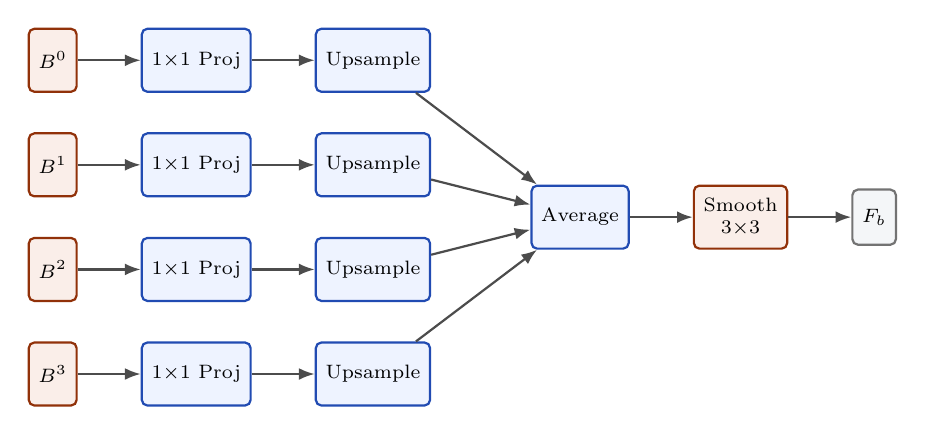
\begin{tikzpicture}[node distance=5mm and 8mm]
        \node[boundary] (b0) {\(B^0\)};
        \node[boundary, below=5mm of b0] (b1) {\(B^1\)};
        \node[boundary, below=5mm of b1] (b2) {\(B^2\)};
        \node[boundary, below=5mm of b2] (b3) {\(B^3\)};

        \node[op, right=of b0] (p0) {\(1{\times}1\) Proj};
        \node[op, right=of b1] (p1) {\(1{\times}1\) Proj};
        \node[op, right=of b2] (p2) {\(1{\times}1\) Proj};
        \node[op, right=of b3] (p3) {\(1{\times}1\) Proj};

        \node[op, right=of p0] (u0) {Upsample};
        \node[op, right=of p1] (u1) {Upsample};
        \node[op, right=of p2] (u2) {Upsample};
        \node[op, right=of p3] (u3) {Upsample};

        \node[op, right=20mm of $(u1)!0.5!(u2)$] (avg) {Average};
        \node[boundary, right=of avg] (smooth) {Smooth\\\(3{\times}3\)};
        \node[tensor, right=of smooth] (bf) {\(F_b\)};

        \foreach \a/\b in {b0/p0,b1/p1,b2/p2,b3/p3,p0/u0,p1/u1,p2/u2,p3/u3}
            \draw[flowarrow] (\a) -- (\b);
        \foreach \u in {u0,u1,u2,u3}
            \draw[flowarrow] (\u) -- (avg);
        \draw[flowarrow] (avg) -- (smooth);
        \draw[flowarrow] (smooth) -- (bf);
    \end{tikzpicture}
    \end{adjustbox}

    \vspace{0.2em}
    \small
    \[
    Q^s=\operatorname{Up}(\operatorname{Proj}_{b,s}^{1\times1}(B^s);H,W),\qquad
    F_b=\operatorname{Smooth}\left(\frac{1}{4}\sum_{s=0}^{3}Q^s\right).
    \]
\end{frame}

\begin{frame}{5.2 Sobel Operator for Coarse Probability}
    \begin{columns}[T,onlytextwidth]
        \begin{column}{0.50\textwidth}
            \centering
            \begin{adjustbox}{max width=\textwidth,max height=0.50\textheight}
            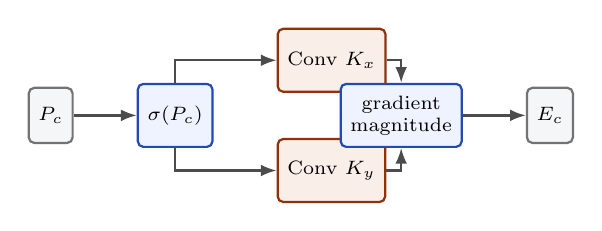
\begin{tikzpicture}[node distance=7mm and 8mm]
                \node[tensor] (pc) {\(P_c\)};
                \node[op, right=of pc] (sig) {\(\sigma(P_c)\)};
                \node[boundary, right=of sig, yshift=7mm] (kx) {Conv \(K_x\)};
                \node[boundary, right=of sig, yshift=-7mm] (ky) {Conv \(K_y\)};
                \node[op, right=16mm of sig] (mag) {gradient\\magnitude};
                \node[tensor, right=of mag] (edge) {\(E_c\)};
                \draw[flowarrow] (pc) -- (sig);
                \draw[flowarrow] (sig) |- (kx);
                \draw[flowarrow] (sig) |- (ky);
                \draw[flowarrow] (kx) -| (mag);
                \draw[flowarrow] (ky) -| (mag);
                \draw[flowarrow] (mag) -- (edge);
            \end{tikzpicture}
            \end{adjustbox}
        \end{column}
        \begin{column}{0.47\textwidth}
            \small
            \[
            P=\sigma(P_c),\qquad
            G_x=P*K_x,\qquad
            G_y=P*K_y.
            \]
            \[
            E_c=\sqrt{G_x^2+G_y^2+10^{-6}}.
            \]
            \scriptsize This Sobel block is single-channel and is applied to the coarse change probability, not to the RGB image.
        \end{column}
    \end{columns}
\end{frame}

\begin{frame}{5.3 Refinement Head}
    \centering
    \begin{adjustbox}{max width=\textwidth,max height=0.49\textheight}
    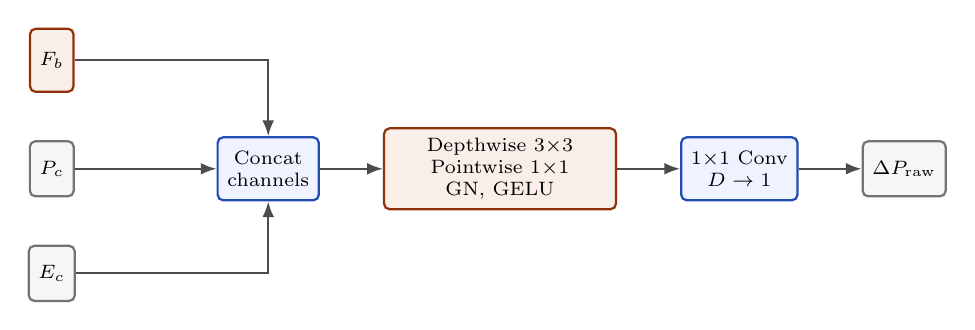
\begin{tikzpicture}[node distance=7mm and 8mm]
        \node[boundary] (bf) {\(F_b\)};
        \node[tensor, below=6mm of bf] (pc) {\(P_c\)};
        \node[tensor, below=6mm of pc] (edge) {\(E_c\)};
        \node[op, right=18mm of pc] (cat) {Concat\\channels};
        \node[boundary, right=of cat, text width=27mm] (dw) {Depthwise \(3{\times}3\)\\Pointwise \(1{\times}1\)\\GN, GELU};
        \node[op, right=of dw] (c1) {\(1{\times}1\) Conv\\\(D\to1\)};
        \node[tensor, right=of c1] (raw) {\(\Delta P_{\mathrm{raw}}\)};

        \draw[flowarrow] (bf) -| (cat);
        \draw[flowarrow] (pc) -- (cat);
        \draw[flowarrow] (edge) -| (cat);
        \draw[flowarrow] (cat) -- (dw);
        \draw[flowarrow] (dw) -- (c1);
        \draw[flowarrow] (c1) -- (raw);
    \end{tikzpicture}
    \end{adjustbox}

    \vspace{0.25em}
    \small
    \[
    X_r=[F_b;P_c;E_c]\in\mathbb{R}^{B\times(D+2)\times H\times W},
    \]
    \[
    H_r=\operatorname{GELU}(\operatorname{GN}(W_{\mathrm{pw}}^{1\times1}*(W_{\mathrm{dw}}^{3\times3}*X_r))),\qquad
    \Delta P_{\mathrm{raw}}=W_\Delta^{1\times1}*H_r+b_\Delta.
    \]
\end{frame}

\begin{frame}{5.4 Elementwise Addition Block}
    \centering
    \begin{adjustbox}{max width=\textwidth,max height=0.42\textheight}
    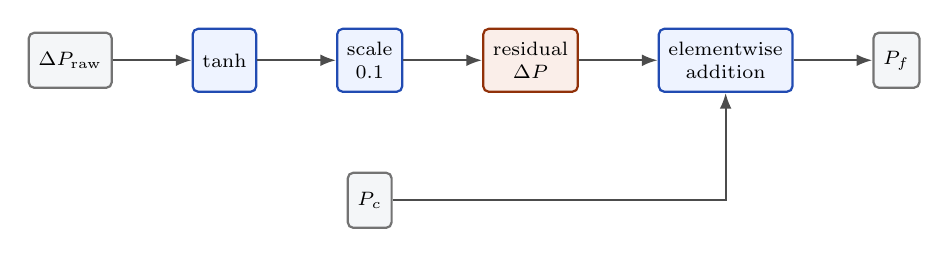
\begin{tikzpicture}[node distance=8mm and 10mm]
        \node[tensor] (raw) {\(\Delta P_{\mathrm{raw}}\)};
        \node[op, right=of raw] (tanh) {\(\tanh\)};
        \node[op, right=of tanh] (scale) {scale\\0.1};
        \node[boundary, right=of scale] (res) {residual\\\(\Delta P\)};
        \node[tensor, below=10mm of scale] (pc) {\(P_c\)};
        \node[op, right=of res] (add) {elementwise\\addition};
        \node[tensor, right=of add] (pf) {\(P_f\)};

        \draw[flowarrow] (raw) -- (tanh);
        \draw[flowarrow] (tanh) -- (scale);
        \draw[flowarrow] (scale) -- (res);
        \draw[flowarrow] (res) -- (add);
        \draw[flowarrow] (pc) -| (add);
        \draw[flowarrow] (add) -- (pf);
    \end{tikzpicture}
    \end{adjustbox}

    \vspace{0.4em}
    \small
    \[
    \Delta P=0.1\tanh(\Delta P_{\mathrm{raw}}),\qquad
    P_f=P_c+\Delta P.
    \]
    \scriptsize The residual is bounded in logit space, so refinement can sharpen boundaries without rewriting the coarse region prediction.
\end{frame}

\begin{frame}{Loss Functions}
    The model is supervised at multiple stages:
    
    $$ \mathcal{L} = \mathcal{L}_{\text{BCE}} + \mathcal{L}_{\text{Dice}} + 0.4\mathcal{L}_{\text{coarse}} + 0.1\mathcal{L}_{\text{boundary}} $$
    
    \begin{itemize}
        \item \textbf{Main Loss:} BCE and Dice supervise the final prediction $z_f$.
        \item \textbf{Coarse Loss:} Stabilizes the main region decoder.
        \item \textbf{Boundary Loss:} Uses a Sobel-edge $l_1$ loss to force contour consistency.
    \end{itemize}
\end{frame}

% =============================================================================
\section{Main Results}
% =============================================================================

\begin{frame}{Main Test Results}
    \centering
    \scriptsize
    \begin{tabular}{llrrrrr}
        \toprule
        \textbf{Dataset} & \textbf{Model} & \textbf{Pre.} & \textbf{Rec.} & \textbf{F1} & \textbf{IoU} & \textbf{OA} \\
        \midrule
        DSIFN-CD & MambaRefine-CD & 95.47 & 95.87 & \textbf{95.67} & \textbf{91.71} & 96.98 \\
        WHU-CD & MambaRefine-CD & 95.79 & 94.90 & \textbf{95.34} & \textbf{91.10} & 99.56 \\
        WHU-CD & MambaRefine-CD VMamba & 96.32 & 94.68 & \textbf{95.49} & \textbf{91.37} & 99.57 \\
        \bottomrule
    \end{tabular}

    \vspace{0.8em}
    \begin{columns}[T,onlytextwidth]
        \begin{column}{0.48\textwidth}
            \small
            \textbf{What this says}
            \begin{itemize}
                \item DSIFN reaches 95.67 F1 and 91.71 IoU on the clean split.
                \item WHU reaches 95.34 F1 / 91.10 IoU with the MambaRefine-CD result summary.
                \item The VMamba variant gives the best WHU score: 95.49 F1 / 91.37 IoU.
            \end{itemize}
        \end{column}
        \begin{column}{0.49\textwidth}
            \small
            \textbf{Evaluation rule}
            \begin{itemize}
                \item Test metrics use the EMA/best checkpoint selected by validation F1.
                \item The threshold is selected from \(\{0.30,0.35,\ldots,0.60\}\).
                \item DSIFN split integrity was verified as PASS; no train/test overlap.
            \end{itemize}
        \end{column}
    \end{columns}
\end{frame}

\begin{frame}{Dataset and Training Protocol}
    \begin{columns}[T,onlytextwidth]
        \begin{column}{0.48\textwidth}
            \small
            \textbf{Data}
            \begin{itemize}
                \item DSIFN-CD: 2758 train, 394 val, 789 test images.
                \item DSIFN test: 3156 tiles at \(256\times256\), overlap \(0.25\).
                \item WHU-CD: standard train/val/test split.
            \end{itemize}

            \vspace{0.4em}
            \textbf{Inference}
            \begin{itemize}
                \item Patch-based inference with crop \(256\).
                \item Validation every 5000 iterations.
                \item Final mask: \(\hat{Y}=\mathbb{1}[\sigma(P_f)>\tau^\star]\).
            \end{itemize}
        \end{column}
        \begin{column}{0.49\textwidth}
            \scriptsize
            \begin{tabular}{ll}
                \toprule
                \textbf{Setting} & \textbf{Value} \\
                \midrule
                Optimizer & AdamW \\
                Learning rate & \(5\times10^{-5}\) \\
                LR schedule & cosine decay \\
                Warmup & 2500 iters \\
                Weight decay & 0.01 \\
                Grad clip & 0.5 \\
                Batch / image & 8 / \(256\times256\) \\
                Precision & AMP BF16/FP16 \\
                EMA decay & 0.999 \\
                Augmentation & horizontal + vertical flip \\
                \bottomrule
            \end{tabular}
        \end{column}
    \end{columns}
\end{frame}

\begin{frame}{Metric Equations}
    \small
    Let changed pixels be the positive class after thresholding
    \(\hat{Y}=\mathbb{1}[\sigma(P_f)>\tau]\). With \(\epsilon=10^{-6}\):

    \vspace{-0.2em}
    \begin{align*}
    \mathrm{Precision} &= \frac{TP}{TP+FP+\epsilon}\times100, &
    \mathrm{Recall} &= \frac{TP}{TP+FN+\epsilon}\times100,\\
    \mathrm{F1} &= \frac{2\,\mathrm{Precision}\,\mathrm{Recall}}
    {\mathrm{Precision}+\mathrm{Recall}+\epsilon}, &
    \mathrm{IoU} &= \frac{TP}{TP+FP+FN+\epsilon}\times100,\\
    \mathrm{OA} &= \frac{TP+TN}{TP+TN+FP+FN+\epsilon}\times100.
    \end{align*}

    \vspace{0.3em}
    \textbf{Boundary metrics}
    \[
    \mathrm{BF1}=\frac{2P_bR_b}{P_b+R_b+\epsilon},\qquad
    \mathrm{BIoU}=\frac{|B_{\mathrm{pred}}\cap B_{\mathrm{gt}}|}
    {|B_{\mathrm{pred}}\cup B_{\mathrm{gt}}|+\epsilon}\times100.
    \]
    \scriptsize
    \(BF1\), \(BIoU\), and Trimap F1 are computed on edge/trimap regions, so they measure contour alignment rather than only changed-area overlap.
\end{frame}

% =============================================================================
\section{Conclusion}
% =============================================================================

\begin{frame}{Conclusion}
    \begin{itemize}
        \item \textbf{Main result:} DSIFN-CD reaches 95.67 F1 / 91.71 IoU; WHU-CD reaches 95.34 F1 / 91.10 IoU, with the VMamba variant at 95.49 F1 / 91.37 IoU.
        \item \textbf{Mechanism:} MambaVision gives the major region gain; signed D-RBI and ARF-FPN provide smaller but measurable additions.
        \item \textbf{Boundary value:} A1 \(\rightarrow\) A6 improves BF1 by 10.58 points and BIoU by 8.98 points in boundary evaluation.
        \item \textbf{Practical choice:} MambaVision-S is the best completed accuracy/complexity trade-off; larger backbones show diminishing returns.
    \end{itemize}
\end{frame}

\begin{frame}[standout]
    Questions? \\
    \vspace{1em}
    \normalsize Thank you for your time.
\end{frame}


\end{document}
